\pagestyle{fancy}
\fancyhf{}
\fancyfoot[L]{\textbf{ECEN 4638--T.D. Murphey}}
\fancyfoot[R]{\textbf{Lab \#1}}
\fancyfoot[C]{\vspace{.2in}\thepage}
%\pagestyle{myheadings}
%\markright{ECEN 4638--T.D. Murphey \flushright Lab $\#1$}


\chapter{Lab \#1:  Introduction to Digital Simulation in LabVIEW}
\date{}
\maketitle
\thispagestyle{fancy}
%\thispagestyle{empty}

\begin{center}  \textbf{Objective}
\end{center}

The purpose of this lab is to become familiar with using the graphical
programming language provided by LabVIEW (or other similar languages such as
SIMULINK) for simulation and implementation of digital control systems.  The
main steps in this lab will be the following.  First, you will simulate a linear
model of the torsional disk system with only one disk and that is using a
proportional controller.  You will then include the effects of saturation and
time delays in your model.  Lastly, you will implement a proportional controller
on your simulated system.  Before doing any of this, you will need to be
comfortable with the LabVIEW programming environment, so you may wish to look at
the tutorial that will be available on \emph{http://moodle.cs.colorado.edu}. You
may alternatively wish to go to www.ni.com and look at one of their interactive
tutorials.  Lastly, a PDF of a user's guide for LabVIEW should be on the lab
computers at \textbf{Start$>>$Programs$>>$National Instruments$>>$LabVIEW
  8.2$>>$Search the LabVIEW Bookshelf.pdf}.

\section{Tasks}

\begin{figure}[h!]
\centering
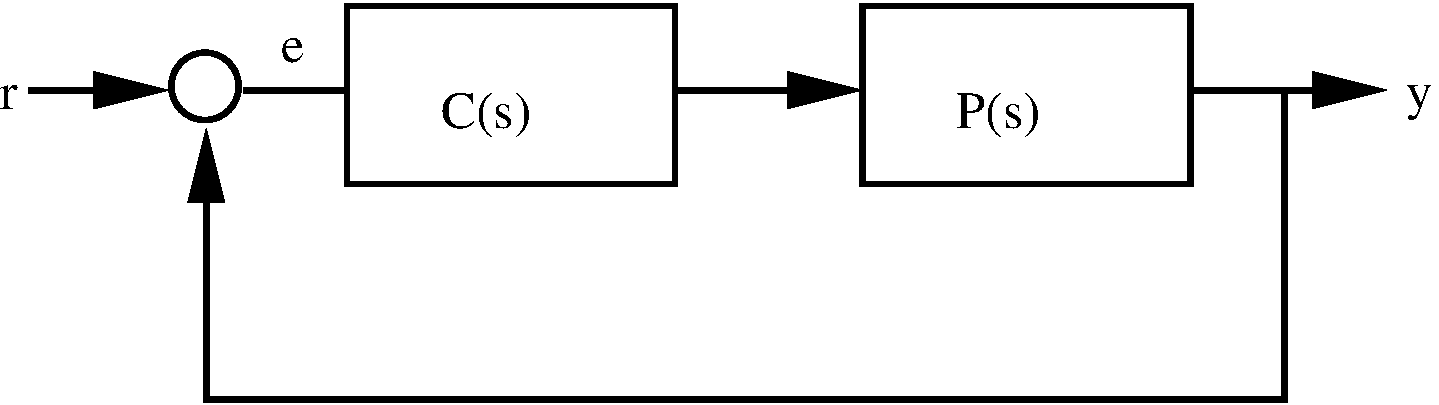
\includegraphics[width=4in]{Lab1/prelimfig1.pdf}
\label{fig-blockdiaglab1}
\end{figure}

In this lab we will be considering a second-order mechanical system.  For now,
assume the system is linear and can be represented as a feedback loop (seen in
Fig.\ref{fig-blockdiaglab1}).  Assume that $C(s)=K_p$ and
$P(s)=\frac{K}{s^2+2\zeta\omega s+\omega^2}$.  This will be the \emph{idealized} plant for
the torsional disk system with only one disk.  For this lab, use the parameter
values $K=1, \zeta=1.25,$ and $\omega=2$.


\subsection{Task \#1--Step Response}

Examine the response of the system to a step response of 10 for 30 seconds.
(You may shorten this length of time if it will be helpful.)  Find the maximum
value of $K_p$ that results in $0\%$ and $50\%$ overshoot.  Record how long it
takes to get within $2\%$ of the desired state (the \emph{$2\%$ settling time})
and how long it takes to get within the \emph{steady state error} for both
cases.  Lastly, what are the \emph{units} in this block diagram?  Label each
wire of the block diagram with its physical units.  What does a step response of
``10'' mean physically?

For each case, turn in a plot that includes the \emph{output}, the \emph{step
  input}, and the \emph{controller} input.  (These can typically be copied
directly from LabVIEW to MS Word.  Plot control can be obtained by right
clicking on the plot and choosing options.)

\subsection{Task \#2--Actuator Saturation}

Although we model many systems as being linear, most are actually nonlinear.
One of the most common nonlinearities that one can encounter is a
\emph{saturation}.  All actuators have saturations because they cannot actually
provide infinite force or torque.  Use the LabVIEW saturation block to insert a
saturation on the control in your simulation.  Start with an step reference of
size 1, and create a saturation of $-200$ to $200$ on the output of your control
block, and then decrement it until you start to see the effects in your
simulation.

Using the same gains determined in Task \#1, record the $2\%$ settling time and
the steady state error for a step size of $1$.  Then do so again for a step size
of $10$.  How does this change your results?  Obtain the same plots as requested
in Task \#1.  

\subsection{Task \#3--Time Delay}

Time delays are another problem in many control systems.  Insert a time delay in
the feedback loop to represent processing time for the sensors.  At what time
delay do you start seeing what you would deem ``significant'' difficulties?  

\subsection{Task \#4--''Best'' $K_p$}

What do you think is the ``best'' $K_p$ for this system if there are saturations
and/or time delays?  Defend your answer using the plots and data you have
accumulated during the rest of the exercise.  

\subsection{Task \#5--Dependence on $\omega$}

What happens if you change $\omega$?  In particular, what happens if you change it to
$0$ or to $10$?  How does this affect your performance/stability/etc?


\section{Things You May Want To Know}

All of the vi's that you need to complete this lab are part of LabVIEW's
Simulation Module.  Hopefully, the LabVIEW tutorial from class has been
sufficient.  However, a copy of the Simulation Module manual is available online
at www.ni.com.  Searching ``Simulation Module'' within this site will bring you
to the pdf manual.  Alternatively, you may wish to view Finn Haugen's website at
\emph{http://www.techteach.no/publications/labview/}.



\vspace{0.2in}
         

\noindent Remember, if you get stuck on some part of the lab, ask your
classmates, the TA, or myself.


%% Local Variables:
%% TeX-master: "../LVmanual.tex"
%% End:
